\section{Auswertung}
In diesem Kapitel sollen die aufgenommenen Messwerte ausgewertet werden.
Über die Schaltung wurden zudem noch folgende Werte notiert:
\begin{center}
    $L = 16,78 +/- 0,09 \si[]{mH}$,\\
    $C = 2,066 +/- 0,006 \si[]{nF}$,\\
    $R = 67,2 +/- 0,2 \si[]{\Omega}$.\\
\end{center}
\subsection{Berechnung der Abklingdauer}
\label{sec:abklingdauer}
Die aufgenommenen Wertepaare aus Spannung $U(t)$ und $t$ wurden in \autoref{fig:bild1}
aufgetragen und es wurde eine Ausgleichskurve hindurchgelegt. Sie hat die Parameter:
\begin{center}
    
        $a = 3.3568 \pm 0.0669 \Leftrightarrow U_0 = 3.3568 \pm 0.0669 \si{\volt}$ \\
        $b = -1119.1751 \pm 100.4186 \Leftrightarrow \mu = 178.1222 \pm 15.982 \si{\per\second}$ .\\
    
\end{center}  
Der erste Parameter kann hier als Spannung $a=U_0$ interpretiert werden.
Über die Beziehung 
\begin{center}
    $R_{eff} = 4\pi\mu L = -2 L b$
\end{center}


lässt sich der Dämpfungswiderstand $R_{eff}$, mit $L = 16,78 \pm 0,09 \si{mH}$ zu
\begin{center}
    $R_{eff} = 37.6 \pm 3.4 \si{\ohm}$
\end{center}
bestimmen. Damit lässt sich über \autoref{eq:prozentuale} die prozentuale Abweichung des gemessenen
gegenüer des Verbauten Widerstandes $R = 67,2 \pm 0,2  \si{\Omega}$ zu $44\pm 5 \si{\percent}$ bestimmen.
Nun kann auch die Abklingdauer mithilfe des Zusammenhangs
\begin{center}
    $T_{ex} = - \frac{1}{b}$
\end{center}
berechnet werden. Damit folgt sofort:
\begin{center}
    $T_{ex} = 0.00089\pm 0.00008 \si[]{s}$. \\
\end{center}

\begin{figure}
    \centering
    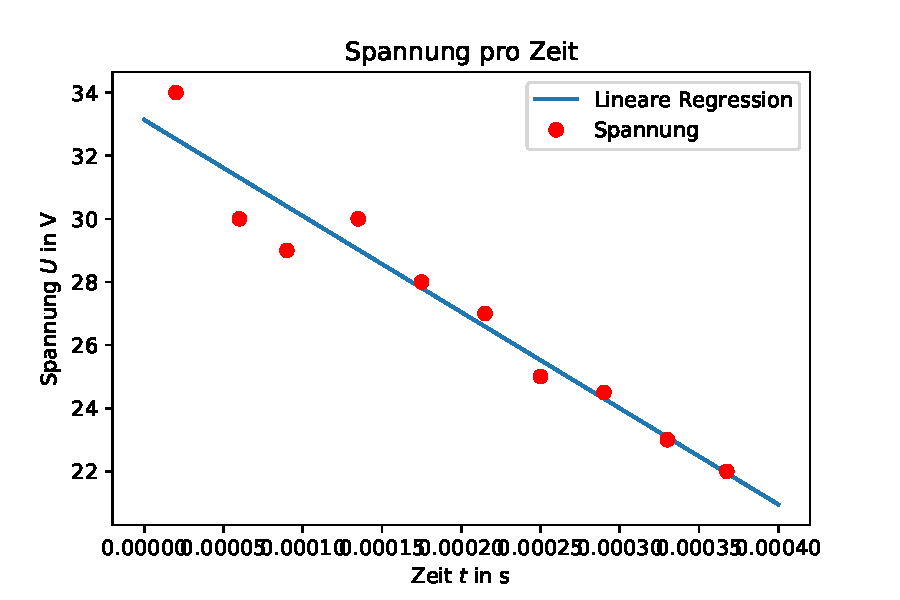
\includegraphics{spannungsverlauf.pdf}
    \caption{Spannungsverlauf in der Zeit}
    \label{fig:bild1}
  \end{figure}

  \subsection{Der Aperiodische Grezfall}
  Der Widerstand wurde solange verändert bis der Aperiodische Grenzfall eingetreten ist. Der zu diesem 
  Zeitpunkt eingestellte Widerstand liegt bei:
  \begin{center}
      $R_{ap}=\SI[]{2.91}[]{k\Omega}$.\\
  \end{center}
  Der entsprechende Widerstand lässt sich mit den gegebenen für $L$ und $c$ Werten auch über:
  \begin{center}
      $R_{ap}=2\sqrt{\frac{L}{C}}=5,700+/-0,017\si[]{k\Omega}$
  \end{center}
  bestimmen. Die nach \autoref{sec:prozentuale} berechnete prozentuale Abweichung beträgt 48.94\%.
  Sie lässt sich vorallem dadurch erklären das es schwirig ist exakt den richtigen Widerstand 
  einzustellen da das eintreten des Aperiodischengrenzfalls nur schwer auf dem Osziloskop zu erkennen  ist,
  es handelt sich also um einen Ablesefehler. Erschwerend kommt hinzu das Verschiedene Widerstände von Leitungen
  und Innenwiderstände von Geräten wie dem Oszilloskop und dem Erreger nicht ideal sind.

  \subsection{Resonanzüberhöhung}
  In \autoref{fig:resonanz}
  \begin{figure}
    \centering
    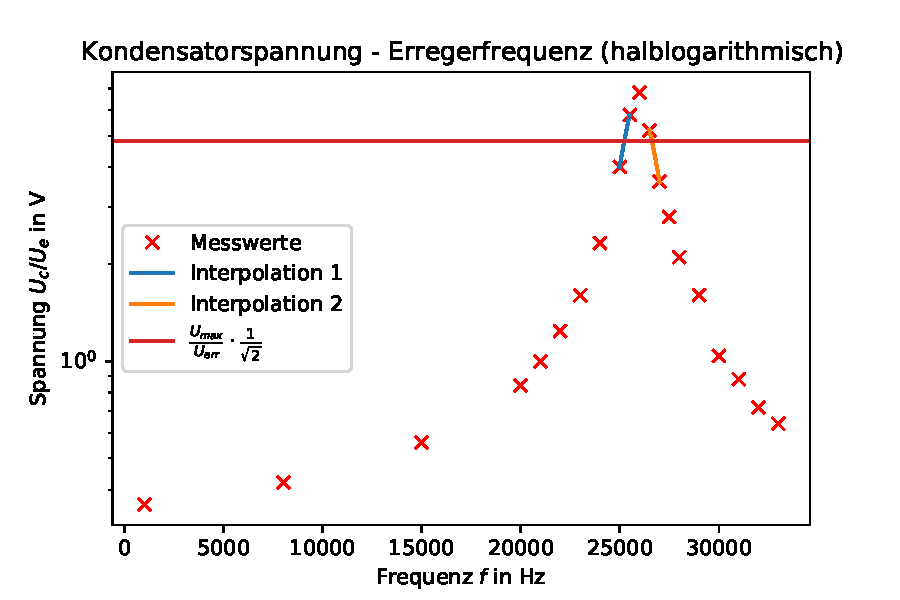
\includegraphics{frequenz.pdf}
    \caption{Spannungsverlauf in Abhängigkeit der Frequenz}
    \label{fig:resonanz}
  \end{figure}
%%%%%%%%%%%%%%%%%%%%%%%%%%%%%%%%%%%%%%%%%%%%%%%%%%%%%%%%%%%%%%%%%%%%%%%%%%%%%%%%%%%%%%
  \section{Auswertung}













\subsection{Frequenzabhängigkeit der Kondensatorspannung}

Die gemessene Kondensatorspannung $U_C$ und die dazugehörige Frequenz $\omega$ wird in die \autoref{tab:2} eingetragen und 
der Quotient $\frac{U_C}{U_\text{Err}}$ gegen die Frequenz $\omega$ halblogarithmisch in die Abbildung (9) aufgetragen.



\begin{figure}
    \centering
    \includegraphics{Daten/c.pdf}
    \label{fig:21}
    \caption{Quotient $\frac{U_C}{U_\text{Err}}$ gegen die Frequenz $\omega$ halblogarithmisch aufgetragen}
\end{figure}


\noindent
Aus der Grafik lässt sich für die Frequenzen, bei denen die Spannung den Wert $\frac{U_\text{max}}{U_\text{Err}}\frac{1}{\sqrt{2}}$ erreicht, entnehmen als

\begin{align*}
    \omega_+ &= 35,1 \pm 0,3 \,  \si{\kilo\hertz} \\
    \omega_- &= 38,5 \pm 0,3 \,  \si{\kilo\hertz} \, .
\end{align*}

\noindent
Daraus folgt die Breite 
\begin{equation*}
    b = 3,4 \pm 0,3 \si{\kilo\hertz} \, .
\end{equation*}

\noindent
Für die Güte kann mit der \autoref{eqn:guete} $$ q = 70 \pm 6 \, $$ berechnet werden. 

\noindent
Die theoretische Breite der Ressonanzkurve lässt sich der \autoref{eqn:wmp} nähern. Mithilfe dieser Näherung lässt sich die Breite der Ressonanzkurve und die Güte berechnen zu %w+ - w- = R/L

\begin{align*}
    b & = 8.657 \pm 0.025 \, \si{\kilo\hertz}\\
    q & = 27.61\pm 0.04 \, . 
\end{align*}

\noindent
Daraus folgt für den Fehler zwischen der theoretischen und gemessen Güte ein Fehler von $1.55 \pm 0.22 \si{\percent}$.